%%%%%%%%%%%%%%%%%%%%%%%%%%%%%%%%%%%%%%%%%%%%
%%%%%%%% Edison abado Ancco
%%%%%%%%%%%%%%%%%%%%%%%%%%%%%%%%%%%%%%%%5555
\documentclass[11pt]{article}
\usepackage[spanish]{babel}
\decimalpoint
\usepackage[utf8]{inputenc}
\usepackage{amsmath}
\usepackage{listings}
\usepackage[usenames]{color} %seteamos el uso de nombre y color
\definecolor{gray97}{gray}{.97}%definimos nombre y color
\usepackage{textcomp}
\lstset{
	frame=Ltb,
	framerule=1pt,
	framextopmargin=5pt, %margen de arriba
	framexbottommargin=5pt, %margen de abajo
	framexleftmargin= 2pt, %separacion del margen izquierdo
	framesep=5pt,
	rulesep=0.3pt,
	backgroundcolor=\color{gray97},
	rulesepcolor=,
	tabsize=2,
	rulecolor=\color[RGB]{106, 182, 217}, %AZUL
	upquote=true,
	aboveskip={2\baselineskip}, %despues de la linea de texto
	columns=fixed,
	showstringspaces=false,
	extendedchars=true,
	breaklines=true,
	prebreak = \raisebox{0ex}[0ex][0ex]{\ensuremath{\hookleftarrow}},
	showtabs=false,
	showspaces=false,
	showstringspaces=false,
	basicstyle=\scriptsize\ttfamily\color[RGB]{39, 100, 46}, %Numeros de lineas, simbolos, puntos y coma y demas
	identifierstyle=\ttfamily\color[RGB]{56, 140, 189}, %variables
	commentstyle=\color[RGB]{62, 179, 101}, %comentarios
	stringstyle=\color[RGB]{247, 165, 42}, %impresiones
	keywordstyle=\bfseries\color[RGB]{237, 118, 150}, %funciones
	%
	numbers=left,
	numbersep=1pt, %separacion del numero
	numberstyle=\tiny,
	numberfirstline = false,
	breaklines=true,
}
\usepackage{textcomp}
\usepackage{graphicx}
\usepackage[colorinlistoftodos]{todonotes}
\usepackage{eso-pic}
\usepackage{avant}
%\usepackage[a4paper]{geometry}
\usepackage[top=1.8cm,bottom=1.8cm,left=1.8cm,right=1.8cm,headsep=8pt,a4paper]{geometry}
\usepackage{fancyhdr}
\pagestyle{fancy}
\fancyhf{}
%\fancyhead[LE,RO]{UNSAAC 2019-II}
%\fancyhead[RE,LO]{Ingenieria Electrónica}
%\fancyfoot[CE,CO]{\leftmark}
\fancyfoot[CO]{\thepage}
\renewcommand{\headrulewidth}{1pt}
\renewcommand{\footrulewidth}{1pt}
\usepackage{tabu}
\usepackage{array}
\usepackage{multirow}
\usepackage{amssymb}
\usepackage{makeidx}
\usepackage{wrapfig}
\usepackage{enumerate}
\usepackage{amsmath,tikz}
\usepackage{steinmetz}
\newcommand*{\horzbar}{\rule[0.05ex]{2.5ex}{0.5pt}}
\usepackage{calc}
\usepackage{dsfont}
\usepackage{enumitem}
\usepackage{subfig}
\usepackage[american]{circuitikz} %también se puede definir por cada circuito poniendo [american] después de {circuitikz}
%\usepackage[siunitx, RPvoltages]{circuitikz}

\usepackage{pgfplots}
\pgfplotsset{compat = newest}

\title{
	\textsc{Universidad Nacional de San Antonio Abad del Cusco}\\
	\textbf{Compuertas Lógicas}\\
	Preinforme 1}

\author{
	\begin{tabular}{lr}
		Edison \textsc{Abado Ancco} & 145012 \\
	\end{tabular}
}


\begin{document}
	\begin{titlepage}
		\newcommand{\HRule}{\rule{\linewidth}{0.5mm}} 
		\center
		\textsc{\LARGE \vspace{1.8cm} \\ Universidad Nacional de San \\[0.2cm] Antonio Abad del Cusco}\\[1.2cm] 
		
\includegraphics[width=3cm]{IMAGENES/escudo}\\[1cm]
		\textsc{\Large Facultad de Ingeniería Eléctrica, \\ Electrónica, Informática y Mecánica}\\[0.5cm] 
		\textsc{\large Escuela Profesional de Ingeniería Electrónica}\\[0.5cm]
		\textsc{\Large \textbf{Circuitos Electrónicos II}}\\[0.5cm] 
%		\textsc{\huge Informe Final}\\[0.2cm]
		\HRule \\[0.4cm]
		{ \huge \bfseries Amplificador Diferencial con alguna aplicación}\\[0.30cm] 
		\HRule \\[1.4cm]
		\begin{minipage}{\textwidth}
			\center 
			
			\emph{Docente:} \\
			Prof. Franklin  \textsc{Cardeñoso Fernandez} \\[1cm]
			
			\begin{tabular}{c}
				\emph{Alumnos:}  \\
				Edison   \textsc{Abado Ancco} - 145012 \\
				Alumno 2 \\
				Alumno 3
			\end{tabular}
		\end{minipage}\\[2cm]
		\today
	\end{titlepage}
	
	
\newpage
	
%\tableofcontents indice bloqueado xD
	
\setlength{\parindent}{0pt} % Stop paragraph indentation
	
\section{Introducción}

Cito \cite{Oppenheim}

\begin{figure}[h!]
	\centering
	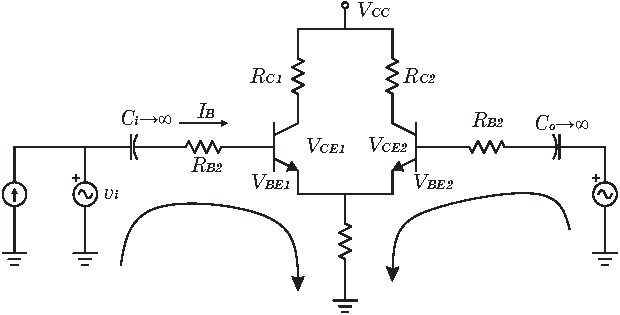
\includegraphics[scale=1]{IMAGENES/prueba1}
	\caption{Descrición de la imgameg 1}
	\label{img1}
\end{figure}




%%%%%%%%%%%%%%%%%%%%%%%%%%%%%%5
%% BIBLIOGRAFÍA %%%
%%%%%%%%%%%%%%%%%%%%%%%%%%%%%%%

\bibliographystyle{ieeetr}
\bibliography{bibliografia}

	
	
\end{document}
